\begin{figure}[H]
\centering
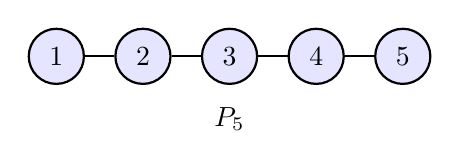
\begin{tikzpicture}[
  vnode/.style={circle, draw, minimum size=7mm, inner sep=0pt, fill=blue!10},
  thick
]
  \foreach \i in {1,2,3,4,5} {
    \node[vnode] (v\i) at ({(\i-1)*1.1}, 0) {\i};
  }
  \draw (v1) -- (v2) -- (v3) -- (v4) -- (v5);
  
  \node at (2.2, -0.8) {$P_5$};
\end{tikzpicture}
\caption{Cesta $P_5$ s pěti vrcholy.}
\end{figure}